\documentclass{sig-alternate}

\setcopyright{acmcopyright}

\usepackage{color}
% \usepackage{hyperref}
\usepackage{graphicx}
\usepackage{multicol}
\usepackage{tikz}
\usepackage{amsfonts}
\usepackage{pgfplots} % to draw axis
\pgfplotsset{compat=1.13}
% \usepackage{amsthm}
\newtheorem{definition}{Definition}



\conferenceinfo{WSDM '17}{February 6--19, 2013, Cambridge, UK}


\begin{document}

\title{Estimating the Lifetime Potential of Scholars\\ \textit{\Large Draft} }

\numberofauthors{2}

\author{
% 1st. author
\alignauthor
Qi Feng\\
       \affaddr{New York University}\\
       \affaddr{New York, NY}\\
       \email{qf264@nyu.edu}
% 2nd. author
\alignauthor
Panos Ipeirotis\\
       \affaddr{New York University}\\
       \affaddr{New York, NY}\\
       \email{panos@nyu.edu}
}

\maketitle

\begin{abstract}
We present a technique for predicting the future performance of academic scholars. Our method models each scholar as a two dimensional sequence, one dimension capturing the production of individual publications from the scholar and the second dimension captures the impact of each publication over time. Based on our model, we present a predictive method that estimates the lifetime potential of each scholar. Using a comprehensive data set that contains faculty members from the top-20 universities in the US, across all fields, we demonstrate that our model can predict with high accuracy the future career trajectories of scholars, even in a 30-year horizon.
\end{abstract}

\keywords{citation analysis; }

\section{Introduction}
Scientific research is becoming more and more influencing and has been creating a large collection of publications, especially in the past 50 years.
Google Scholar service went online on November 20 2004, and is estimated to hold the metadata for roughly 8.7 million publications as of May 2016\cite{}.
The growing size of publications over years is shown in figure \ref{publicationcount-year}.
\begin{figure}
\begin{center}
\resizebox {\columnwidth} {!} {

\begin{tikzpicture}
\begin{axis}[
	xlabel = Year,
	ylabel = Number of publication,
]

\addplot[color=blue] table[x={year}, y={count}]{data/publication-year};
\end{axis}
\end{tikzpicture}
}
\caption{Number of publications over year on Google Scholar.}
\label{publicationcount-year}
\end{center}
\end{figure}

Predicting the impact of a publication meets the needs of researchers. The impact of a publication is conventionally represented by the number of citations over the years.
However, research institutions and organizations are more interested on predicting and evaluating the overall performance of a researcher in the next several years.

The influence of a researcher may result from multiple publication from wide range of fields or might from a single milestone publication that revolutionized the whole field as well. However, the influence is time variant. The popularity of a researcher will change over time. This might result from the popularity of a research field or a new theory come into the filed.
The most direct and widely adopted evaluation of a researcher's scholar influence is his or her total citation counts. The number of citations and h-index can reflect the scholar and performance of a researcher in a lifetime scale\cite{bornmann2007we}. However, these indicators does not necessarily reflect a researchers recent and current scholar performance. Therefore, the number of citations in a short period of time is a better indicator of the recent scholar performance and influence of a researcher.

Since the citations of publications shows a power law distribution, traditional regressions commonly gives poor results from publication citation data\cite{cheng2014can,radicchi2008universality}. 

In our work, future citations counts are used as an indicator for research performance and popularity of a researcher. Our prediction task is to formulate a regression model for the number of citations a researcher get during a given time frame, based on the historical citation data and other author related features. We will present a unique two stage approach to formulate a prediction model on future citation counts for researchers. As we shall see in our work, the predicted future citations of publications will contribute a positive factor in predicting future citation counts for a researcher.

To give a better prediction, a regression model for individual publications is first formulated, which is majorly based on Yan et al's work\cite{yan2011citation}. This model is then utilized to generate a predicted future citations of a researcher based on all publications he or she published before the given time.
\section{Related Works}
Modeling research performance has been explored in many different approaches, especially in modeling indicators of future research performance and predicting these indicators over time. Studies on research performance prediction offer research organizations more general ways to evaluate the potential research performance of a researcher in coming years.

Conventionally, the influence and popularity of publications are measured by the number of citations, typically by overall total citations for influence and yearly citations for recent popularity. Extensive works have been done on predicting citations of publications.

Total number of citations of an individual publication prediction based on historical citations has been studied in 2003 ACM SIGKDD Competition \cite{gehrke2003overview}. Predicting total number of citations is categorized in social network mining. Perlich and Provost proposed a statistical model technique with aggregation operators that capture more information about the value distributions, by storing meta-data about value distributions and referencing this meta-data when aggregating\cite{perlich2003aggregation}. Predicting the total citations of an individual publication will provide a general sense of the lifetime influence of the given publication but barely reflect its recent popularity.

A citation count prediction learning framework of publications is proposed by Yan et al.\cite{yan2011citation}. In their work, several publication related features alongside author features are chosen to predict the number of citations of publications in the next fixed number of years. They achieved a regression coefficient of determination($R^2$) at 0.75 for predicting citations in the next 5 years, with a classification and regression tree(CART) model proposed by Breimann in 1984\cite{breiman1984classification}. CART is tested out to performance better in this regression problem.

Metrics for evaluating the performance of researchers are introduced over the years. Conventionally, the total number of citations of all publications from an author is used to indicate his or her research performance. However, a researcher lacks productivity may benefit from a well cited publication, which means even though total citations reflects the popularity of a researcher, it does not necessarily reflect the productivity of researchers.
On the contrary, total number of publications published by a researcher reflects the productivity but does not reflect the popularity of a researcher.

Hirsch introduced the h-index, which reflects both the popularity and the productivity of researchers\cite{hirsch2005index}. He also reported that h-index is a more predictive indicator than number of citations and number of publications. H-index, when utilized to predict number of citations and papers in the future, will perform better than number of citations and papers themselves respectively\cite{hirsch2007does}. However, despite its widespread positive reception, some objections are proposed, majorly arguing the multidimensional researchers might suffer from a lower h-index and the performance of researchers should not be evaluated using a single metric\cite{van2006comparison,glanzel2006h,glanzel2006opportunities}.

Google also proposed the i10-index for their Google Scholar service, which counts the number of publications that have a citation count higher than or equal to $10$. i10-index is straight forward but does not used anywhere else except Google Scholar.

With both these index and total citations accepted as a general measurement for research performance, researchers are eager to publish more publications with a higher number of citations.

\section{Problem Definition}
In this section, we will formally define the prediction problem that we solve.
As has been discussed before, predicting total number of citations in the future does not necessarily reflect the recent production and popularity of researchers. Therefore, predicting the number of citations during a given time frame of researchers will give a better sense of the recent productivity and popularity of researchers.

In this paper, we will generalize a new publication-level approach to predict the performance of a researcher in the near future.

Following Yan et al.'s definition\cite{yan2011citation}, the citation of a publication $p$ in a collection of publications $P$ is defined as follows.

\begin{definition}
Given a publication collection $P$, and a publication $p\in P$, the citations of a publication $p$ at time $t$
\[C_T(p,t):=|citing(p,t)|,\]
where
\[citing(p):=\{\forall p'\in P, p' \textit{ cites } p \]
\[\textit{ AND } p' \textit{ is published before } t \}.\]
\end{definition}

We define the number of citations of a researcher as the aggregation of citations of all his or her publications.

\begin{definition}
The number of citations of a researcher $r$ at time(typically year) $t$ in a publication collection $P$
\[N_c(r,t):=\sum_{\forall p \in P(r)} C_T(p,t),\]
where
\[P(r):=\{\forall p \in P, r \textit{ coauthored } p\}.\]
\label{def-author-citations}
\end{definition}

In our perspective, the predicting of citations that is accumulated only in the next few years
will have a stronger representation of a researcher's activeness and potential research performance.
Therefore, our learning task is now defined as follows.

\begin{definition}
Given a set of researcher features, $\vec{X}=x_1,x_2,\cdots,x_n$, our goal is to learn a predictive function $f$ to predict the citation
of a research between time $t$ and some time period $\delta t$ later. Define
\[D_c(r,t,\Delta t):=N_c(r,t+\Delta t)-N_c(r,t)\]
%difference in citations
Formally, we are giving
\[f(r|\vec{X},t,\Delta t)\rightarrow D_c(r,t,\Delta t).\]
\end{definition}

\section{Features}
To generalize the prediction of research performance for researchers, conventional author features are incorporated into the prediction model.
Additionally, a new feature that is given by the prediction from all publications of a researcher is utilized as well.
Details of these chosen features are introduced in this section.

\subsection{Conventional Researcher Features}
\subsubsection{Organization Rank}
The prediction problem for each researcher intuitively depends on the organization of the author themselves, including its rank and authority.
Prior researches have been devoted to examining the relation between citations counts and the rank of researchers' organization\cite{van2005fatal}.

In our model, we will use the rank of the organization alone as a feature to represent the authority of an organization.

\subsubsection{Professorship}
Same reason as the organization rank, professorship should be considered when predicting future citations of a researcher intuitively. Professorships are simplified and divided into four ranks. Professor, Associate Professor, Assistant Professor and others respectively.

\subsubsection{Historical Citations Counts $N_c(r,t)$}
It is important to utilize historical records to predict future in a time series prediction task\cite{weigend1994time}.
Therefore, we add $N_c(r,t_{now})$, $N_c(r,t_{now}-1)$, and $N_c(r,t_{now}-2)$ into our model.
The number of citations within a year (yearly citations) are also included in this model, that is,
citations in current year
$N_c(r,t_{now})-N_c(r,t_{now}-1)$, citations in last year $N_c(r,t_{now}-1)-N_c(r,t_{now}-2)$ and citations in the year before last year $N_c(r,t_{now}-2)-N_c(r,t_{now}-3)$.

\subsubsection{h-index}
As Hirsch pointed out\cite{hirsch2007does}, h-index has a good predictive power for $N_c(r,t)$.
Besides that, h-index, when combined with $N_c(r,t)$, to predict $N_c(r,t+\Delta t)$ are better than the number of papers and the mean citations per paper.
Therefore, we include this feature into our model as a feature combined with historical citation counts to give better prediction for next $\Delta t$ year citation counts.

It is worth notice that the h-index, we used is the h-index for a researcher $r$ in year $t_{now}$.

\subsubsection{i10-index}
The $i10$-index indicates the number of academic publications an author has written that have at least ten citations from others.
It was introduced in July 2011 by Google as part of their work on Google Scholar.\cite{delgado2014google}

As is the same reason as h-index, we will include this feature in our prediction model. $i10$-index is also computed for each researcher in each year.

\subsubsection{Active years}
Active years, that is the number of years since publishing the first paper, is also an important factor to determine the future scientific performance.
As is reported in the {\it Science} paper\cite{acuna2012future}, active years contributes as a negative factor in future h-index.
Same reason here, when predicting the future total citations, it is also reasonable and important to incorporate this feature into the prediction model.

\subsection{Publication-level Prediction}
Following Yan et al.\cite{yan2011citation}, we formulated a prediction model for publication citation prediction and used this model to generate a new feature for researchers.

In our publication citation prediction model, we incorporate the first author's feature, including author's organization rank, h-index, and i10-index, for each publication.
Additionally, the historical citation of the certain publication is also considered to give predictions for the total number of citations of the given publication in the next $\Delta t$ years.
It is important to find regression models which are appropriate for this specific problem.
Linear regression(LR), decision forest regression(DFR), Poisson regression(PR), and regularized LR (namely LASSO and ridge regression) are trained with cross validation in our specific settings.

Finally, a new feature based on this publication-level prediction model is constructed in an intuitive way.

\begin{definition}
The new feature is defined as estimated next $\Delta t$ year citations,

\[\hat{D_c}(r,t,\Delta t):=\sum_{\forall p \in P(r)} \textit{ Predicted number of}\]
\[\textit{citations of } p \textit{ from } t \textit{ to } t+\Delta t.\]
\end{definition}

This new feature is incorporated in the model for a detailed assisting feature for author level citations prediction, since by definition\ref{def-author-citations}, the number of citations of a researcher is the sum of citations of all his or her publications.

\section{Regression Models}
In this section, we will describe regression models that are tested in our experiment.

\subsection{Linear Regression}
Linear Regression is an approach for modeling the relationship between a dependent variable $y$ and explanatory variables $X$ in a scalar way. A linear regression result has an equation of the following form, $Y = AX +b$. In this paper, researcher features are treated as explanatory variables and future citation counts are considered as dependent variable.
\subsection{Random Forest}
Random Forest is an ensemble learning method by constructing a multitude of decision trees during training. The output of a random forest is the mode of classes of individual decision trees.

In our experiments, we used bagging as the re-sample method, since bagging is reported to be resilient to noise features\cite{dietterich2000ensemble}.

We tuned the number of trees and the maximum depth of the trees in $\{103,308,513,718,923\}$.
We tuned the minimum number of re-sampling per leaf in $\{7,20,33,56,59\}$.

\subsection{Boosted Decision Trees}
Gradient boosting trees are an ensemble of decision trees via boosting. Boosting ensembles a series of weak classifiers, decision trees in our case, to formulate a learning model. Gradient boosting builds the model by allowing optimization of an arbitrary differentiable loss function\cite{friedman2002stochastic}.

We tuned the minimum and maximum number of leaves per tree in $\{100,300,500,700,900\}$.
We tuned the number of trees constructed in $\{1000,3000,5000,7000,9000\}$.
We tuned the learning rate in $\{0.1,0.3,0.5,0.7,0.9\}$.

\subsection{Poisson Regression}
Poisson regression is a statistical regression model which assumes a Poisson distribution of the predicting label, i.e. the citation counts in this paper. As mentioned before, the distribution of citations of all authors falls into a Poisson distribution. Therefore, Poisson regression might find a fit in this prediction. However, we assume that Poisson regression will have a worse predicting performance than the previous mentioned ensemble learning methods, since the features in our dataset will not direct form a Poisson distribution on citation counts.

We tuned the l2 regularization parameter in $\{10^{-i}, i = -2,-1,0\}$.
We tuned the l1 regularization parameter in $\{0.0, 0.01, 0.1, 1.0\}$.

\subsection{Ridge Regression}
Regularized linear regression prevents model from over fitting on noisy data sets\cite{mohri2012foundations,tibshirani1996regression}.
We use the ordinary least squares as the optimization method and tuned $\lambda$ in regularization from $\{10^{-i}, i = -2,-1,0,1,2\}.$
\section{Experiments}
\subsection{Data Source}
We perform the researcher future citation prediction on the Google Scholar database.
It covers 3,666,012 publications by 23,140 researchers for more than 50 years.
The total number of citations is 128,157,386 in this data set.

We used all papers with cross validation to formulate the publication level future citation prediction model.
With this model we created a new feature that aggregates all the number of citation predicted from all papers a researcher published before year $t$.

For each researcher who has been active for at least $\Delta t$ years, we generate a new record in a new data set for each year after the first $\Delta t$ years, i.e. if a researcher has been active for 40 years and $\Delta t=5$. 35 records are generated for every year after five years in the field. 

We first clean all records with an N/A value by removing the entire row.
We split the entire data set randomly into two parts, $80\%$ for training and validation and $20\%$ for test.
For the $80\%$ data, we split it into two parts. $75\%$ are used for training and $25\%$ are used for validation.
We select the best hyper parameter using training set and validation set. We then used the best hyper parameter to train a model on both training set and validation set. Finally, we test our model on the test set.

We compare our predicted future citations with actual future citations in the test set.

\subsection{Evaluation}
The coefficient of determination ($R^2$) is used in evaluating how well prediction model fits the test data. Let the set of all researchers be $R$, then the definition of $R^2$ is:
\[R^2=\frac{\sum_{r \in R}(\hat{D_c}(r,t,\Delta t)-f(r|\vec{X},t,\Delta t))^2}{\sum_{r \in R}(\hat{D_c}(r,t,\Delta t)-\bar{D_c}(r,t,\Delta t))^2}\]
where $\hat{D_c}$ is the actual future citation for researcher $r$ in year $t$, $f$ is our prediction
and $\bar{D_c}$ represents the mean of the actual citations from year $t$ to $t+\Delta t$ for all researchers.

By definition, $R^2 \leq 1$, with $R^2=0$ means the predicted citations does not fit the actual citations at all,
and $R^2=1$ means the model perfectly predicted the future citations. A model with a larger $R^2$ indicates a better prediction performance and is therefore desired. 
\subsection{Prediction Performance}
Following Yan et al.'s work, our prediction model for publication future citation is summarized in table \ref{tbl-pubprediction}.

\begin{table}[!h]
\begin{center}
\begin{tabular}{c|c|c|c|c|c}
\hline
$R^2$& LR & DFR & PR & LASSO & Ridge\\
\hline
$\Delta t=1$ & & & & &\\
\hline
$\Delta t=5$ & & & & &\\
\hline
$\Delta t=10$ & & & & &\\
\hline
\end{tabular}
\end{center}
\caption{Publication future citation prediction evaluation}
\label{tbl-pubprediction}

\end{table}

We achieved a much better regression result by performing a data cleaning and using decision forest regression as our model. We then use the trained model to compute the predicted publication future citation counts. Finally, for each author and year, we sum the number of predictions from publication future citation counts prediction as a new feature we discussed above.

The prediction for researcher future citations is summarized in table \ref{tbl-r2}.
The best predictive performance for next five year researcher citations is plotted in figure \ref{author-prediction}.


\begin{figure}
    \centering
    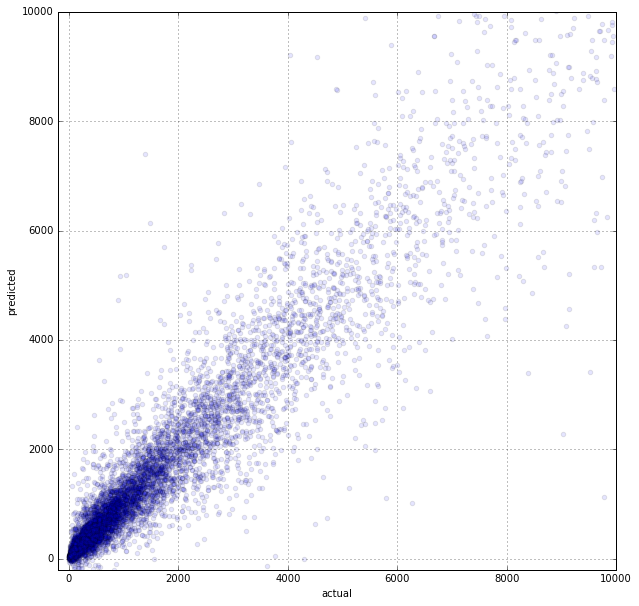
\includegraphics[width=\columnwidth]{fig/author-prediction.png}
    \caption{Author Citations in Next 5 Years, Prediction vs. Actual.}
    \label{author-prediction}
\end{figure}

\begin{table*}[t]
\begin{center}
\begin{tabular}{c|c|c|c|c|c|c|c|c|c|c|c|c|c|c|c}
\hline
& \multicolumn{5}{|c|}{\textbf{$\Delta t =1$}}& \multicolumn{5}{|c|}{$\Delta t =5$}& \multicolumn{5}{|c}{$\Delta t =10$}\\

\hline
Methods & LR & DFR & PR & SVR & R& LR & DFR & PR & SVR & R& LR & DFR & PR & SVR & R\\
\hline\hline
+org.Rank & & & & & & & & & & & & & & & \\
\hline
+$N_c(r,t)$ & & & & & & & & & & & & & & & \\
\hline
+index & & & & & & & & & & & & & & & \\
\hline
+years & & & & & & & & & & & & & & & \\
\hline\hline
-org.Rank & & & & & & & & & & & & & & & \\
\hline
-$N_c(r,t)$ & & & & & & & & & & & & & & & \\
\hline
-index & & & & & & & & & & & & & & & \\
\hline
-years & & & & & & & & & & & & & & & \\
\hline\hline
Combined & & & & & & & & & & & & & & & \\
\hline
\end{tabular}
\end{center}
\caption{The performance of various predictive models on the test set."+""-"}
\label{tbl-r2}

\end{table*}



\subsubsection{Citation Distribution}
As is shown in figure \ref{author-prediction}, the distribution of future researchers citations shows a long tail. 
Most researchers gets a total future citations less than 2,500 cites.
However, even with this long tail distribution, our publication level feature leveages this problem and achieved an overall $R^2$ at $0.957$.

\subsubsection{Factor Contribution}
As we shall see in table \ref{tbl-r2}, three major factors that have a strong impact on the prediction performance are historical citation counts, indexes that represent the performance of research performance and the publication level feature that we introduced before.

Since we are prediction the number of future citation counts of a researcher, both historical yearly citation counts and historical total citation counts are useful features. A simple linear combination of these features forms a good representation of the future citation counts. It is trivial that these historical citation counts feature contributes a big improvement on prediciton performance.

H-index and i-10 index as have been discussed in the previous section will have a good representation on the research performance. Hirsh states that h index has a better prediction property to total citation counts\cite{Hirsh2007does}. However, since we are predicting the future citation counts which is the difference of citation counts between now and the future, H-index and i-10 index are relatively a weaker indicator compared to the historical citation counts.

Our unique feature, the publication level prediction helps improve the prediction performance from $R^2 = 0.750$ to $R^2 = 0.957$ using decision forest regression method. The feature itself can predict the citation count in the next 5 years as good as historical citations. Both the publication level prediction and historical citations performs better than h-index and i10-index combined.

\section{Conclusion}
In this paper, we present a publication level approach for researcher future citations(PLRFC) prediction, which predicts the future total citations for a researcher. 
Our works will also cast some light for predicting the future scholar performance of a researcher.

Our predictive model will fully discover the publication and researcher data set. 

Given a certain researcher and its corresponding features relevant with citation patterns (such as the organization of this researcher, indexes for evaluating the scholar performance etc.), PLRFC predicts the citation counts of all publications of this researcher in the next few years. We formally formulate PLRFC task as a learning problem based on multiple regression models.
Finally, PLRFC prediction model is evaluated by the coefficient of determination ($R^2$).

PLRFC is a two step prediction model. We first formulated a model for publication future citation prediction and utilized this model to generate a new feature of a researcher as the sum of all predicted future citations for all publication of this researcher.
\section{Acknowledgements}


\bibliographystyle{abbrv}
\bibliography{texfiles/bib}

\end{document}


